\documentclass{beamer}
\usepackage{graphicx} 
\usetheme{Warsaw}
\usecolortheme{beaver}
\usepackage{tikz}
\usetikzlibrary{arrows}
\usepackage{amsthm}
\usepackage{fontawesome5}
\usepackage[utf8]{inputenc}
\usepackage[usenames,dvipsnames]{xcolor}
\usepackage[upright]{fourier}
\usepackage{tkz-graph}
\usetikzlibrary {decorations.pathmorphing}
\usetikzlibrary{shapes.geometric, arrows,calc}
\usepackage{fontawesome5}
\usepackage{xcolor}
% \usepackage{enumitem}

% Define TikZ styles for the flowchart elements
\tikzstyle{startstop} = [rectangle, rounded corners, minimum width=3cm, minimum height=1cm,text centered, draw=black, fill=green!30]
\tikzstyle{attack} = [rectangle, rounded corners, minimum width=1.5cm, minimum height=1cm,text centered, draw=black, fill=red!30]
\tikzstyle{retreat} = [rectangle, rounded corners, minimum width=1.2cm, minimum height=1cm,text centered, draw=black, fill=blue!30]
\tikzstyle{process} = [rectangle, minimum width=3cm, minimum height=1cm, text centered, draw=black, fill=orange!30]
\tikzstyle{processDiff} = [rectangle, minimum width=3cm, minimum height=1cm, text centered, draw=black, fill=orange!30]
\tikzstyle{decision} = [diamond, minimum width=3cm, minimum height=1cm, text centered, draw=black, fill=green!30]
\tikzstyle{arrow} = [thick,->,>=stealth]
\definecolor{byzantinePurple}{RGB}{102, 51, 153}
\definecolor{goldAccent}{RGB}{218, 165, 32}
\definecolor{customgreen}{RGB}{33,213,63}

\title{Byzantine General Problems}
\author[Shatabdi \and Shadman \and Roki]{
 2105124- Shadman Abid \and \\
 2105123- Shatabdi Dutta Chowdhury \and \\
 2105129- Sarowar Alam Roki
}
\date{\today}




% Set up the page style and fancy header
\pagestyle{empty} % Removes page numbers and headers
\begin{document}

\frame{\titlepage}

% 2105124 start
\begin{frame}{Introduction}
    
\begin{tikzpicture}

    % Define coordinates
    \node (server1) at (0, 4) {\includegraphics[width=2cm]{image/server.png}};
    \node (processor1) at (4, 4) {\includegraphics[width=2cm]{image/Processor.png}};
    \node (graph1) at (9, 4) {\includegraphics[width=3cm]{image/input.png}};
     \draw[->, thick] (processor1) -- (server1);
    \draw[->, thick] (graph1) -- (processor1);

    \pause
    
     \only<2>{\node[draw=green!80!black, ultra thick, circle, minimum size=1cm, fill=green!30] at (3.7, 4) {\textbf{\checkmark}};}
     
     \pause
     
    \node[draw=red!80!black, ultra thick, circle, minimum size=1cm, fill=red!30] at (3.7, 4) {\textbf{\texttimes}};   
    \only<3>{
    \node (error) at (3, 0) {\includegraphics[width=10cm]{image/not working.png}};
    }
     \only<4>{
      \node (error) at (3, 0) {\includegraphics[width=10cm]{image/connectionerror.png}};
     }
\end{tikzpicture}

 \pause
     \uncover<5,6>{
      \begin{itemize}
        \item The value of Facebook's share dropped by 5. 5\% costing around 7 billion dollars.
      \uncover<6>{   \item And also Amazon lost 528 million dollars }
    \end{itemize}
     }
    
    \uncover<5,6>{
     \begin{tikzpicture}
          \node (sloth) at (13, -1) {\includegraphics[height=2cm]{image/dumbsloth.png}};
    
    % Add speech bubble near the sloth
    \node[draw, callout, callout relative pointer={(-1, 0.5)}, fill=blue!20, rounded corners, text width=4cm] at (10, 0) {
        \textbf{"Wait a second, that's a lot of money, sloth!!!"}
    }
    \end{tikzpicture}
     }
     \uncover<6>{
    \begin{tikzpicture}
        
     \node (character) at (6, -1) {\includegraphics[height=2cm]{image/smartsloth.png}};
    
    % Add speech bubble for the new character
    \node[draw, callout, callout relative pointer={(1, 0.5)}, fill=green!20, rounded corners, text width=3cm] at (4.5, 0) {
        \textbf{"Yep, it is"}
    };
     \end{tikzpicture}
    }
\end{frame}

\begin{frame}{Introduction..}
\begin{tikzpicture}
    \node at (0,0) {\includegraphics[height=7cm]{image/bg.png}}
\end{tikzpicture}
    
\end{frame}
    
\end{frame}

\begin{frame}{The Story Behind...}

\begin{tikzpicture}
    \node [anchor=center](civilPlane) at (0, 4) {\includegraphics[width=2cm]{image/passenger plane.png}};
    \node [anchor=center](radar) at (0, 0) {\includegraphics[width=2cm]{image/radar.png}};
    
    
    \node [anchor=west](stalin) at (4.5,0){\includegraphics[height=2cm]{image/stalin.png}};
    \node[draw, callout, callout relative pointer={(-1, 0.5)}, fill=blue!20, rounded corners, text width=4cm] at (3, 1.5) {
        Hmmm , a white plane with lots of passengers , Seems suspicious!!
    }
     \node [anchor=east](radar2) at (-1,-1){\includegraphics[height=2cm]{image/single.png}};
     
     \pause
    \node [anchor=east](lenin) at (-4,0){\includegraphics[height=2cm]{image/lenin.png}};
    \only<2>{\node[draw, callout, callout relative pointer={(-1, 0.5)}, fill=blue!20, rounded corners, text width=4cm] at (-3, 1.5) {
        And ooh look the radar also says so};}
   \only<3>{
    \node[draw, callout, callout relative pointer={(-1, 0.5)}, fill=blue!20, rounded corners, text width=4cm] at (-3, 1.5) {
        Okay boys , Let's nuke that plane , haha };
   }
   
        
\end{tikzpicture}
    
\end{frame}

\begin{frame}{The Story Behind...}

\begin{tikzpicture}
    \node [anchor=center](fighter) at (0, 4) {\includegraphics[width=3cm]{image/fighter jet.png}};
    \node [anchor=center](radar) at (0, 0) {\includegraphics[width=2cm]{image/radar.png}};
    
    \node [anchor=west](stalin) at (4.5,0){\includegraphics[height=2cm]{image/stalin.png}};
    \node[draw, callout, callout relative pointer={(-1, 0.5)}, fill=blue!20, rounded corners, text width=4cm] at (3, 1.5) {
        Hmm , an F-35 raptor ? Looks good to me !!
    }
     \node [anchor=east](radar2) at (-1,-1){\includegraphics[height=2cm]{image/nothing.png}};
     
     \pause
    \node [anchor=east](charlamagne) at (-4,0){\includegraphics[height=2cm]{image/Charlamagne.png}};
    \uncover<2,3>{\node[draw, callout, callout relative pointer={(-1, 0.5)}, fill=blue!20, rounded corners, text width=4cm] at (-3, 1.5) {
        And Look there's nothing on the radar};}
   \only<3>{
    \node[draw, callout, callout relative pointer={(-1, 0.5)}, fill=blue!20, rounded corners, text width=1cm] at (-2, 4) {
         haha };
   }
   
        
\end{tikzpicture}



    
\end{frame}

\begin{frame}{The Story Behind...}
    \begin{columns} % Begin a columns environment
        \begin{column}{0.5\textwidth} % Set the width of the first column
            \begin{figure}
                \centering
                \includegraphics[width=\linewidth]{image/RobertShoshtack.png}
                \caption{Robert Shoshtack}
            \end{figure}
        \end{column}
        \begin{column}{0.5\textwidth} % Set the width of the second column
           \begin{tikzpicture} % Use TikZ to draw the red square
                \node (image) at (0, 0) {\includegraphics[width=\linewidth]{image/LeslieLamport.png}};
                % Draw a red rectangle around the image
                \pause
                \draw[red, ultra thick] (image.south west) rectangle (image.north east);
            \end{tikzpicture}
        \end{column}
    \end{columns}
\end{frame}

\begin{frame}{Byzantine Generals Problem}
    \framesubtitle{Problem Formulation}
    \begin{columns}
        \begin{column}{.3\textwidth}
         \begin{itemize}
             \item Communication through messages.
             \item Generals must decide upon a plan
             \item \alert{Concensus}
         \end{itemize}
        \end{column}
        \begin{column}{.7\textwidth}
            \begin{tikzpicture}
                % Place the fort image in the center
                \node[anchor=center] (fort) at (0, 0) {\includegraphics[width=2cm]{image/fort.png}};
            
                % Place the general images around the fort
                \node[anchor=center] (general1) at (-3, 2) {\includegraphics[width=2cm]{image/commander.png}};
                \node[anchor=center] (general2) at (3, 2) {\includegraphics[width=2cm]{image/commander.png}};
                \node[anchor=center] (general3) at (-3, -2) {\includegraphics[width=2cm]{image/commander.png}};
                \node[anchor=center] (general4) at (3, -2) {\includegraphics[width=2cm]{image/commander.png}};
            
            \end{tikzpicture}
        \end{column}
    \end{columns}
\end{frame}


\begin{frame}{Byzantine Generals Problem}
    \framesubtitle{Consensus to Attack}
    \begin{columns}
        \begin{column}{.3\textwidth}
    
         \begin{itemize}
             \item \textbf{\textit{\textcolor{Green}{Attack}}} 
         \end{itemize}
        \end{column}
        \begin{column}{.7\textwidth}
            \begin{tikzpicture}
                % Place the fort image in the center
                \node[anchor=center] (fort) at (0, 0) {\includegraphics[width=2cm]{image/fort.png}};
            
                % Place the general images around the fort
                \node[anchor=center] (general1) at (0, 3) {\includegraphics[width=1.5cm]{image/commander.png}};
                \node[anchor=center] (general2) at (3, 0) {\includegraphics[width=1.5cm]{image/commander.png}};
                \node[anchor=center] (general3) at (0, -3) {\includegraphics[width=1.5cm]{image/commander.png}};
                \node[anchor=center] (general4) at (-3, 0) {\includegraphics[width=1.5cm]{image/commander.png}};

                \node at (0, 1.5) {\includegraphics[width=.7cm]{image/down arrow.png}};
                \node at (1.5, 0) {\includegraphics[width=1cm]{image/left arrow.png}};
                \node at (0, -1.5) {\includegraphics[width=.6cm]{image/up arrow.png}};
                \node at (-1.5, 0) {\includegraphics[width=1cm]{image/right arrow.png}};
            
                % Add the speech bubbles with "ATTACK!"
                \node[anchor=west] at (.7, 3) {\includegraphics[width=2cm]{image/attack3.png}};
                \node[anchor=east] at (4, -1.5) {\includegraphics[width=2cm]{image/attack4.png}};
                \node[anchor=west] at (-3, -3) {\includegraphics[width=2cm]{image/attack1.png}};
                \node[anchor=east] at (-1, 1.5) {\includegraphics[width=2cm]{image/attack2.png}};
                        
            \end{tikzpicture}
        \end{column}
    \end{columns}
\end{frame}

\begin{frame}{Byzantine Generals Problem}
    \framesubtitle{Consensus to Retreat}
    \begin{columns}
        \begin{column}{.25\textwidth}
         \begin{itemize}
             \item \textbf{\textit{\textcolor{Red}{Retreat}}} 
         \end{itemize}
        \end{column}
        \begin{column}{.75\textwidth}
            \begin{tikzpicture}
                % Place the fort image in the center
                \node[anchor=center] (fort) at (0, 0) {\includegraphics[width=2cm]{image/fort.png}};
            
                % Place the general images around the fort
                \node[anchor=center] (general1) at (0, 2) {\includegraphics[width=1.5cm]{image/commander.png}};
                \node[anchor=center] (general2) at (2, 0) {\includegraphics[width=1.5cm]{image/commander.png}};
                \node[anchor=center] (general3) at (0, -1.7) {\includegraphics[width=1.5cm]{image/commander.png}};
                \node[anchor=center] (general4) at (-2.5, 0) {\includegraphics[width=1.5cm]{image/commander.png}};

                \node at (0, 3.5) {\includegraphics[width=.7cm]{image/up red arrow.png}};
                \node at (3, 0) {\includegraphics[width=1cm]{image/right red arrow.png}};
                \node at (0, -2.8) {\includegraphics[width=.6cm]{image/down red arrow.png}};
                \node at (-4, 0) {\includegraphics[width=1cm]{image/left red arrow.png}};
            
                % Add the speech bubbles with "ATTACK!"
                \node[anchor=west] at (.7, 2.7) {\includegraphics[width=2cm]{image/Retreat1.png}};
                \node[anchor=east] at (4, -2) {\includegraphics[width=2cm]{image/Retreat2.png}};
                \node[anchor=west] at (-3, -2) {\includegraphics[width=2cm]{image/Retreat3.png}};
                \node[anchor=east] at (-1, 1.5) {\includegraphics[width=2cm]{image/Retreat4.png}};
                        
            \end{tikzpicture}
        \end{column}
    \end{columns}
\end{frame}


\begin{frame}{Byzantine Generals Problem}
    \framesubtitle{Consensus to Attack with  Traitor Included}
    \begin{columns}
        \begin{column}{.3\textwidth}
        \begin{itemize}
            \item  \alert{Traitors}
            \item The \textit{\textcolor{Green}{loyal Generals}} must reach a \textit{\textcolor{Blue}{consensus}} .
        \end{itemize}
        \end{column}
        \begin{column}{.7\textwidth}
            \begin{tikzpicture}
                % Place the fort image in the center
                \node[anchor=center] (fort) at (0, 0) {\includegraphics[width=2cm]{image/fort.png}};
            
                % Place the general images around the fort
                \node[anchor=center] (general1) at (0, 3) {\includegraphics[width=1.5cm]{image/commander.png}};
                \node[anchor=center] (general2) at (3, 0) {\includegraphics[width=1.5cm]{image/commander.png}};
                \node[anchor=center] (general3) at (0, -3) {\includegraphics[width=1.5cm]{image/Traitor.png}};
                \node[anchor=center] (general4_traitor) at (-3, 0) {\includegraphics[width=1.5cm]{image/commander.png}};

                \node at (0, 1.5) {\includegraphics[width=.7cm]{image/down arrow.png}};
                \node at (1.5, 0) {\includegraphics[width=1cm]{image/left arrow.png}};
                \node at (0, -1.5) {\includegraphics[width=.6cm]{image/up arrow.png}};
                \node at (-1.5, 0) {\includegraphics[width=1cm]{image/right arrow.png}};
            
                % Add the speech bubbles with "ATTACK!"
                \node[anchor=west] at (.7, 3) {\includegraphics[width=2cm]{image/attack3.png}};
                \node[anchor=east] at (4, -1.5) {\includegraphics[width=2cm]{image/attack4.png}};
                \node[anchor=west] at (-3, -2) {\includegraphics[width=2cm]{image/attack1.png}};
                \node[anchor=east] at (-1, 1.5) {\includegraphics[width=2cm]{image/attack2.png}};
                        
            \end{tikzpicture}
        \end{column}
    \end{columns}
\end{frame}


\begin{frame}{Byzantine Generals Problem}
    \framesubtitle{Traitor Interfering}
    \begin{columns}
        \begin{column}{.3\textwidth}
        \begin{itemize}
            \item Traitors can act arbitrarily .
            % \item   Still , the \textit{\textcolor{Green}{loyal Generals}} must reach a \textit{\textcolor{Blue}{consensus}} and act upon that .
        \end{itemize}
        \end{column}
        \begin{column}{.7\textwidth}
            \begin{tikzpicture}
                % Place the fort image in the center
                \node[anchor=center] (fort) at (0, 0) {\includegraphics[width=2cm]{image/fort.png}};
            
                % Place the general images around the fort
                \node[anchor=center] (general1) at (0, 3) {\includegraphics[width=1.5cm]{image/commander.png}};
                \node[anchor=center] (general2) at (3, 0) {\includegraphics[width=1.5cm]{image/commander.png}};
                \node[anchor=center] (general3) at (0, -2) {\includegraphics[width=1.5cm]{image/Traitor.png}};
                \node[anchor=center] (general4_traitor) at (-3, 0) {\includegraphics[width=1.5cm]{image/commander.png}};

                \node at (0, 1.5) {\includegraphics[width=.7cm]{image/down arrow.png}};
                \node at (1.5, 0) {\includegraphics[width=1cm]{image/left arrow.png}};
                \node at (0, -3) {\includegraphics[width=.6cm]{image/down red arrow.png}};
                \draw[->, red, thick, >=latex, line width=1.5pt] (0.7, -2) -- (2.5, -0.6) node[midway, above, sloped, red] {Let's Retreat};
                \node at (-1.5, 0) {\includegraphics[width=1cm]{image/right arrow.png}};
            
                % Add the speech bubbles with "ATTACK!"
                \node[anchor=west] at (.7, 3) {\includegraphics[width=2cm]{image/attack3.png}};
                \node[anchor=east] at (4, -1.5) {\includegraphics[width=2cm]{image/attack4.png}};
                \node[anchor=west] at (-3, -2) {\includegraphics[width=2cm]{image/Retreat3.png}};
                \node[anchor=east] at (-1, 1.5) {\includegraphics[width=2cm]{image/attack2.png}};
                        
            \end{tikzpicture}
        \end{column}
    \end{columns}
\end{frame}



\begin{frame}{Byzantine Generals Problem}
    \framesubtitle{Traitor is Successful}
    \begin{columns}
        \begin{column}{.3\textwidth}
        \begin{itemize}
            \item  A traitor can easily foil any effective strategy if he is not dealt with.
            % \item Even though traitors act arbitrarily , the Generals must impose a system to reach a desired cons
            % ensus.
        \end{itemize}
        \end{column}
        \begin{column}{.7\textwidth}
            \begin{tikzpicture}
                % Place the fort image in the center
                \node[anchor=center] (fort) at (0, 0) {\includegraphics[width=2cm]{image/fort.png}};
            
                % Place the general images around the fort
                \node[anchor=center] (general1_dead) at (0, 3) {\includegraphics[width=1.5cm]{image/Dead.png}};
                \node[anchor=center] (general2) at (2, 0) {\includegraphics[width=1.5cm]{image/commander.png}};
                \node[anchor=center] (general3_traitor) at (0, -2) {\includegraphics[width=1.5cm]{image/Traitor.png}};
                \node[anchor=center] (general4_dead) at (-3, 0) {\includegraphics[width=1.5cm]{image/Dead.png}};

                \node at (0, 1.5) {\includegraphics[width=1cm]{image/down arrow.png}};
                \node at (3, 0) {\includegraphics[width=1cm]{image/right red arrow.png}};
                \node at (0, -3) {\includegraphics[width=1cm]{image/down red arrow.png}};
               
                \node at (-1.5, 0) {\includegraphics[width=1cm]{image/right arrow.png}};
            
                % Add the speech bubbles with "ATTACK!"
                \node[anchor=west] at (.7, 3) {\includegraphics[width=2cm]{image/Opps1.png}};
                \node[anchor=east] at (4, -2) {\includegraphics[width=2cm]{image/Question.png}};
                \node[anchor=west] at (-3, -2) {\includegraphics[width=2cm]{image/haha.png}};
                \node[anchor=east] at (-1, 1.5) {\includegraphics[width=2cm]{image/Opps4.png}};
                        
            \end{tikzpicture}
        \end{column}
    \end{columns}
\end{frame}

\begin{frame}{Relevance of Byzantine Generals Problem to Computer Science..}
\begin{tikzpicture}
    \node[anchor=center](processor1) at (0,0){\includegraphics[height=2cm]{image/Processor.png}}
    \node[anchor=center](processor2) at (0,2){\includegraphics[height=2cm]{image/Processor.png}}    
    \node[anchor=center](processor3) at (0,-2){\includegraphics[height=2cm]{image/Processor.png}}

    \node[anchor=east](server1) at (-3,0) {\includegraphics[height=2cm]{image/server.png}}

    \node[anchor=west](graph1) at (3,0) {\includegraphics[height=2cm]{image/input.png}}
     % Draw different lines (arrows) from input to processors
        \draw[->, thick, blue] (graph1) -- (processor1); % line from input to processor 1
        \draw[->, thick, green] (graph1) -- (processor2); % line from input to processor 2
        \draw[->, thick, orange] (graph1) -- (processor3); % line from input to processor 3

        % Draw lines from processors to the server
        \draw[->, thick, red] (processor1) -- (server1); % line from processor 1 to server
        \draw[->, thick, purple] (processor2) -- (server1); % line from processor 2 to server
        \draw[->, thick, brown] (processor3) -- (server1); % line from processor 3 to server
        \pause
        \node[draw=green!80!black, ultra thick, circle, minimum size=1cm, fill=green!30] at (0, 2) {\textbf{\checkmark}}; % 
        \node[draw=green!80!black, ultra thick, circle, minimum size=1cm, fill=green!30] at (0, -2) {\textbf{\checkmark}}; % 
        \pause
         \node[draw=red!80!black, ultra thick, circle, minimum size=1cm, fill=red!30] at (0, 0) {\textbf{\texttimes}}; % 
\end{tikzpicture}
   \only<4>{Same goes for radars and sensitive identification technology.} 
\end{frame}


%2105124 end

% 2105123 start
\begin{frame}{The Problem Revisited...}
\begin{alertblock}{The Byzantine Generals Problem}
 The \textbf{Byzantine Generals Problem} is a way to understand how computer systems can agree on a decision, even when some parts might not work correctly or try to deceive others. 
 \end{alertblock}
 \end{frame}
 \begin{frame}
 \begin{itemize}
     \item 
      We can relate it with the situation where \textcolor{byzantinePurple}{how a group of generals, represented as computer nodes or processes, must agree on a decision (e.g.,
      whether to \textcolor{red}{attack or retreat}), despite the presence of traitors among them.}
       \end{itemize}
 \end{frame}

\begin{frame}{A Simplified Version}
\begin{columns} 
         \column{0.5\textwidth} 
         There are a total of \textcolor{red}{n} officers on the battlefield.

\column{0.5\textwidth}  
        \begin{figure}
            \includegraphics[width=\textwidth]{images2/museums-victoria-kfmpzG39ndk-unsplash.jpg}
            \caption{Battlefield Scenario with Generals}
        \end{figure}
\end{columns}
\end{frame}
\begin{frame}{A Simplified Version...}
    \begin{columns}
    \vspace{3cm}
         \column{0.5\textwidth} 
         There are a total of \textcolor{red}{n} officers on the battlefield.
        \begin{itemize}
            \item One officer is the \textbf{commanding general}, who will send order to the remaining \textcolor{red}{n-1} are \textbf{lieutenant generals} such that
            \begin{itemize}
                \item \textbf{Condition 1:} All \textcolor{customgreen}{loyal} lieutenants must obey the same order.
                \item \textbf{Condition 2:} If the \textcolor{blue}{commanding general} is \textcolor{customgreen}{loyal}, all loyal lieutenants must follow the order he sends.
            \end{itemize}
        \end{itemize}
        \column{0.5\textwidth}  
        \begin{figure}
            \includegraphics[width=\textwidth]{images2/army-8749314_1280.jpg}  % Replace with the path to your image file
            \caption{Battlefield Scenario with Generals}
        \end{figure}
    \end{columns}
\end{frame}


\begin{frame}{On the way of solution...}
\begin{alertblock}{What is Byzantine generals problem}
    \begin{itemize}
        \item \only<1>{All loyal lieutenants obey the same order.}
              \only<2>{Consistency/Agreement}
              \only<3>{Consistency/Agreement}
              \only<4>{Consistency/Agreement}
         
        \item \only<1>{If the commanding general is loyal, then every loyal lieutenant obeys the order he sends.}
        \only<2>{If the commanding general is loyal, then every loyal lieutenant obeys the order he sends.}
      
         \only<3>{\textbf{\textcolor{black}{If the commanding general is loyal}}, then every loyal lieutenant obeys the order he sends.}
         \only<4>{Validity}
    \end{itemize}    
\end{alertblock}   
\end{frame}

\begin{frame}{On the way of solution...}
\begin{alertblock}{What is Byzantine generals problem}
    \begin{itemize}
        \item {Consistency/Agreement}
        \item {Validity}
        \item {Termination}

    \end{itemize}    
\end{alertblock}   
\end{frame}

\begin{frame}[plain]
    \begin{center}
        \vfill
        {\color{red!70!black}\Huge \textbf{\textsc{Impossibility Result}}}
       
        \rule{\linewidth}{1pt}
        \vfill
    \end{center}
\end{frame}


\begin{frame}{Impossibility Result}
    Now we will go through two main strategies.
    \begin{itemize}
        \item Oral messages
        \item Signed messages
    \end{itemize}
\end{frame}

\begin{frame}{Impossibility Result: Oral Messages}
“if the generals can send only \textcolor{red}{oral messages}, then no solution will work unless more than \textcolor{red}{$\frac{2}{3}$} of the generals are loyal.”
\end{frame}


\begin{frame}{\textbf{Oral Messages}}
    \begin{align*}
        {\color{red}\fontsize{15pt}{24pt}\selectfont \textbf{What are ORAL MESSAGES ???}} 
        \hspace{0.5cm}
        \includegraphics[height=2.5cm]{images2/Screenshot 2024-12-06 014823.png}
    \end{align*}
\end{frame}

\begin{frame}[plain]
    \begin{center}
        \vfill
        {\color{red!70!black}\Huge \textbf{\textsc{A Possible Scenerio}}}
       
        \rule{\linewidth}{1pt}
        \vfill
    \end{center}
\end{frame}



\begin{frame}{Flowchart possibility Result}
    \begin{center}
        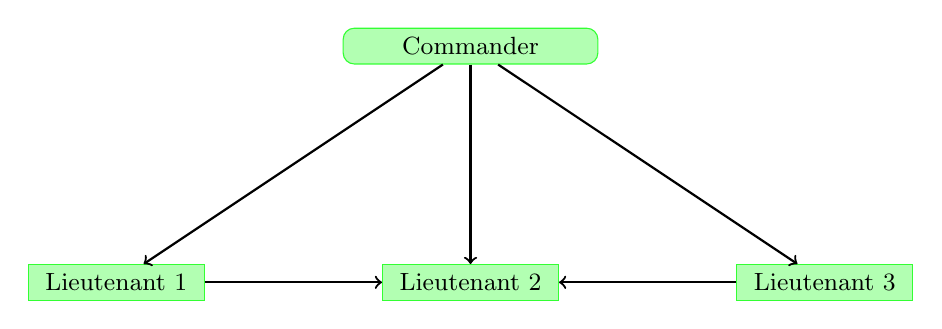
\begin{tikzpicture}[
            node distance=3cm, 
            every node/.style={text centered, font=\small},
            startstop/.style={rectangle, rounded corners, draw=green!80, fill=green!30, text width=3cm},
            process/.style={rectangle, draw=green!80, fill=green!30, text width=2cm}
        ]
            % Nodes
            \node (start) [startstop] {Commander};
            \node (process1) [process, below of=start, xshift=0cm] {Lieutenant 2};
            \node (process2a) [process, below of=start, xshift=-4.5cm] {Lieutenant 1};
            \node (process2b) [process, below of=start, xshift=4.5cm] {Lieutenant 3};

            % Arrows
            \draw [->, thick] (start) -- (process2a);
            \draw [->, thick] (start) -- (process1) ;
            \draw [->, thick] (start) -- (process2b) ;
            \draw [->, thick] (process2a) -- (process1) ;
            \draw [->, thick] (process2b) -- (process1);
        \end{tikzpicture}
    \end{center}
\end{frame}


\begin{frame}{Flowchart Possibility Result}
    \begin{center}
        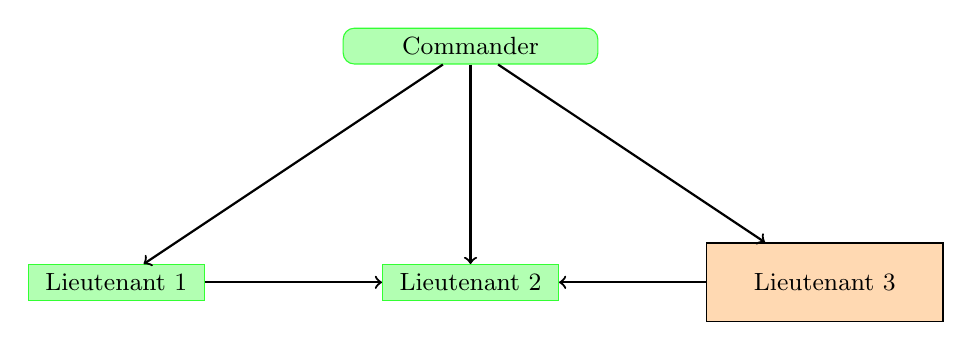
\begin{tikzpicture}[
            node distance=3cm, 
            every node/.style={text centered, font=\small},
            startstop/.style={rectangle, rounded corners, draw=green!80, fill=green!30, text width=3cm},
            process/.style={rectangle, draw=green!80, fill=green!30, text width=2cm}
        ]
            % Nodes
            \node (start) [startstop] {Commander};
            \node (process1) [process, below of=start, xshift=0cm] {Lieutenant 2};
            \node (process2a) [process, below of=start, xshift=-4.5cm] {Lieutenant 1};
            \node (process2b) [processDiff, below of=start, xshift=4.5cm] {Lieutenant 3};

            % Arrows
            \draw [->, thick] (start) -- (process2a);
            \draw [->, thick] (start) -- (process1) ;
            \draw [->, thick] (start) -- (process2b) ;
            \draw [->, thick] (process2a) -- (process1) ;
            \draw [->, thick] (process2b) -- (process1);
        \end{tikzpicture}
    \end{center}
\end{frame}


\begin{frame}{Flowchart Possibility Result}
    \begin{center}
        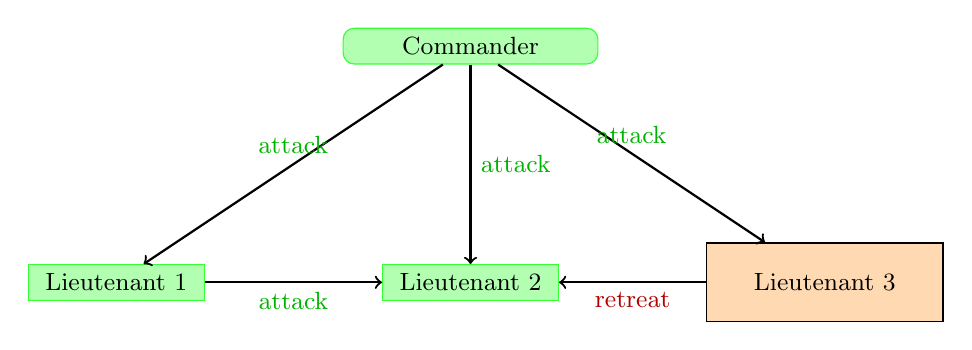
\begin{tikzpicture}[
            node distance=3cm, 
            every node/.style={text centered, font=\small},
            startstop/.style={rectangle, rounded corners, draw=green!80, fill=green!30, text width=3cm},
            process/.style={rectangle, draw=green!80, fill=green!30, text width=2cm}
        ]
            % Nodes
            \node (start) [startstop] {Commander};
            \node (process1) [process, below of=start, xshift=0cm] {Lieutenant 2};
            \node (process2a) [process, below of=start, xshift=-4.5cm] {Lieutenant 1};
            \node (process2b) [processDiff, below of=start, xshift=4.5cm] {Lieutenant 3};

            % Arrows
            \draw [->, thick] (start) -- (process2a) node[midway, above] {\textcolor{green!70!black}{attack}};
            \draw [->, thick] (start) -- (process1) node[midway, right] {\textcolor{green!70!black}{attack}};
            \draw [->, thick] (start) -- (process2b) node[midway, above] {\textcolor{green!70!black}{attack}};\pause
            \draw [->, thick] (process2a) -- (process1) node[midway, below] {\textcolor{green!70!black}{attack}};\pause
            \draw [->, thick] (process2b) -- (process1) node[midway, below] {\textcolor{red!70!black}{retreat}};
        \end{tikzpicture}
    \end{center}
\end{frame}


\begin{frame}{Impossiblity Proof}
  When only one of the generals or the commander is traitor.So the traitor is only one memeber. So the member , \textcolor{red}{m=1}   
\end{frame}
\begin{frame}{Impossibility Result Proof[ \textcolor{red}{m=1}]}
    \begin{center} % Center the entire content
        \begin{tikzpicture}
            % Slide 1: All loyal
            \only<1>{
                \node[anchor=center] (commander) at (0,2) {\includegraphics[width=2cm]{images2/commander.png}};
                \node[anchor=center] (general1) at (-2,-1) {\includegraphics[width=2cm]{images2/soldier (1).png}};
                \node[anchor=center] (general2) at (2,-1) {\includegraphics[width=2cm]{images2/soldier (1).png}};
            }
            % Slide 2: One traitor
            \only<2>{
                \node[anchor=center] (commander) at (0,2) {\includegraphics[width=2cm]{images2/commander.png}};
                \node[anchor=center] (general1) at (-2,-1) {\includegraphics[width=2cm]{images2/soldier (1).png}};
                \node[anchor=center] (general2) at (2,-1) {\includegraphics[width=2cm]{images2/mask (1).png}};
            }
            % Slide 3: Add attack and retreat arrows
            \only<3>{
                \node[anchor=center] (commander) at (0,2) {\includegraphics[width=2cm]{images2/commander.png}};
                \node[anchor=center] (general1) at (-2,-1) {\includegraphics[width=2cm]{images2/soldier (1).png}};
                \node[anchor=center] (general2) at (2,-1) {\includegraphics[width=2cm]{images2/mask (1).png}};
                \draw[->, thick, green!70!black] (commander) -- (general1) node[midway, above] {Attack};
                \draw[->, thick, green!70!black] (commander) -- (general2) node[midway, above] {Attack};
                \draw[->, thick, red!70!black] (general2) -- (general1) node[midway, below] {Retreat};
            }
            % Slide 4: Commander is a traitor
            \only<4>{
                \node[anchor=center] (commander) at (0,2) {\includegraphics[width=2cm]{images2/mask (1).png}};
                \node[anchor=center] (general1) at (-2,-1) {\includegraphics[width=2cm]{images2/soldier (1).png}};
                \node[anchor=center] (general2) at (2,-1) {\includegraphics[width=2cm]{images2/soldier (1).png}};
                \draw[->, thick, green!70!black] (commander) -- (general1) node[midway, above] {Attack};
                \draw[->, thick, red!70!black] (commander) -- (general2) node[midway, above] {Retreat};
                \draw[->, thick, red!70!black] (general2) -- (general1) node[midway, below] {Retreat};
                \draw[->, thick, green!70!black] ([yshift=-1cm]general1.south) -- ([yshift=-1cm]general2.south) node[midway, below] {Attack};
            }
        \end{tikzpicture}
    \end{center}
\end{frame}



\begin{frame}{Three Scenarios [\textcolor{red}{m=1}]}
\begin{columns}
    % First Column
    \column{0.3\textwidth}
    \begin{tikzpicture}
        \node[anchor=center] (commander) at (0,3) {\includegraphics[width=1cm]{images2/commander.png}};
        \node[anchor=center] (general1) at (-1, 0) {\includegraphics[width=1cm]{images2/soldier (1).png}};
        \node[anchor=center] (general2) at (1, 0) {\includegraphics[width=1cm]{images2/mask (1).png}};
        \draw [->, thick] (commander) -- (general1) node[midway, above] {\textcolor{green!70!black}{attack}};
        \draw [->, thick] (commander) -- (general2) node[midway, north] {\textcolor{green!70!black}{attack}};
        \draw [->, thick] (general2) -- (general1) node[midway, below, align=center] {The\\ commander said\\ \textcolor{red!70!black}{retreat}};
    \end{tikzpicture}

    % Vertical Line Between Columns
    \column{0.02\textwidth}
    
\begin{tikzpicture}
        \draw[thick, orange] (0, 3) -- (0, -2); % Adjust height of the vertical line as needed
    \end{tikzpicture}

    % Second Column
    \column{0.3\textwidth}
    \begin{tikzpicture}
        \node[anchor=center] (commander) at (1,3) {\includegraphics[width=1cm]{images2/commander.png}};
        \node[anchor=center] (general2) at (0, 0) {\includegraphics[width=1cm]{images2/mask (1).png}};
        \node[anchor=center] (general1) at (2, 0) {\includegraphics[width=1cm]{images2/soldier (1).png}};
        \draw [->, thick] (commander) -- (general1) node[midway, north] {\textcolor{green!70!black}{attack}};
        \draw [->, thick] (commander) -- (general2) node[midway, above] {\textcolor{green!70!black}{attack}};
        \draw [->, thick] (general2) -- (general1) node[midway, below, align=center] {The\\ commander said\\ \textcolor{red!70!black}{retreat}};
    \end{tikzpicture}

    % Vertical Line Between Columns
    \column{0.02\textwidth}
    
\begin{tikzpicture}
        \draw[thick, orange] (0, 3) -- (0, -2); % Adjust height of the vertical line as needed
    \end{tikzpicture}

    % Third Column
    \column{0.3\textwidth}
    \begin{tikzpicture}
        \node[anchor=center] (commander) at (-1,2) {\includegraphics[width=1cm]{images2/mask (1).png}};
        \node[anchor=center] (general1) at (-1, -2) {\includegraphics[width=1cm]{images2/soldier (1).png}};
        \node[anchor=center] (general2) at (1, -2) {\includegraphics[width=1cm]{images2/soldier (1).png}};
        \draw [->, thick] (commander) -- (general1) node[midway, north] {\textcolor{green!70!black}{attack}};
        \draw [->, thick] (commander) -- (general2) node[midway, above] {\textcolor{red!70!black}{retreat}};
        \draw [->, thick, red] (general2) -- (general1) node[midway, below, align=center] {The\\ commander said\\ \textcolor{red!70!black}{retreat}};
        \draw [->, thick, green!80!black] ([yshift=-1cm]general1.south) -- ([yshift=-1cm]general2.south) 
            node[midway, below, align=center] {The\\ commander said\\ \textcolor{green!70!black}{attack}};
    \end{tikzpicture}
\end{columns}
\end{frame}


\begin{frame}{Three Scenarios}
\begin{columns}
    % First Column
    \column{0.3\textwidth}
    \begin{tikzpicture}
        \node[anchor=center] (commander) at (0,3) {\includegraphics[width=1cm]{images2/commander.png}};
        \node[anchor=center] (general1) at (-1, 0) {\includegraphics[width=1cm]{images2/soldier (1).png}};
        \node[anchor=center] (general2) at (1, 0) {\includegraphics[width=1cm]{images2/mask (1).png}};
        \draw [->, thick] (commander) -- (general1) node[midway, above] {\textcolor{green!70!black}{attack}};
        \draw [->, thick] (commander) -- (general2) node[midway, north] {\textcolor{green!70!black}{attack}};
        \draw [->, thick] (general2) -- (general1) node[midway, below, align=center] {The\\ commander said\\ \textcolor{red!70!black}{retreat}};
       
        \node (attack) [attack, below of=general1, yshift=-2cm,scale=0.5] {ATTACK};
        \draw [->, blue] (general1)--(attack);
    \end{tikzpicture}

    % Vertical Line Between Columns
    \column{0.02\textwidth}
    
\begin{tikzpicture}
        \draw[thick, orange] (0, 3) -- (0, -2); % Adjust height of the vertical line as needed
    \end{tikzpicture}

    % Second Column
    \column{0.3\textwidth}
    \begin{tikzpicture}
        \node[anchor=center] (commander) at (1,3) {\includegraphics[width=1cm]{images2/commander.png}};
        \node[anchor=center] (general2) at (0, 0) {\includegraphics[width=1cm]{images2/mask (1).png}};
        \node[anchor=center] (general1) at (2, 0) {\includegraphics[width=1cm]{images2/soldier (1).png}};
        \draw [->, thick] (commander) -- (general1) node[midway, north] {\textcolor{green!70!black}{attack}};
        \draw [->, thick] (commander) -- (general2) node[midway, above] {\textcolor{green!70!black}{attack}};
        \draw [->, thick] (general2) -- (general1) node[midway, below, align=center,scale=0.5] {The\\ commander said\\ \textcolor{red!70!black}{retreat}};
        \node (retreat) [retreat, below of=general1, yshift=-2cm,scale=0.5] {RETREAT};
        \draw [->, blue] (general1)--(retreat);
    \end{tikzpicture}

    % Vertical Line Between Columns
    \column{0.02\textwidth}
    
\begin{tikzpicture}
        \draw[thick, orange] (0, 3) -- (0, -2); % Adjust height of the vertical line as needed
    \end{tikzpicture}

    % Third Column
    \column{0.3\textwidth}
    \begin{tikzpicture}
        \node[anchor=center] (commander) at (-1,2) {\includegraphics[width=1cm]{images2/mask (1).png}};
        \node[anchor=center] (general1) at (-1, -2) {\includegraphics[width=1cm]{images2/soldier (1).png}};
        \node[anchor=center] (general2) at (1, -2) {\includegraphics[width=1cm]{images2/soldier (1).png}};
        \draw [->, thick] (commander) -- (general1) node[midway, north] {\textcolor{green!70!black}{attack}};
        \draw [->, thick] (commander) -- (general2) node[midway, above] {\textcolor{red!70!black}{retreat}};
        \draw [->, thick, red] (general2) -- (general1) node[midway, below, align=center] {The\\ commander said\\ \textcolor{red!70!black}{retreat}};
        \draw [->, thick, green!80!black] ([yshift=-1cm]general1.south) -- ([yshift=-1cm]general2.south) 
        node[midway, below, align=center] {The\\ commander said\\ \textcolor{green!70!black}{attack}};
        \node (retreat) [retreat, below of=general2.north, yshift=-3cm,scale=0.5] {RETREAT};
        \draw [->, blue] (general2)--(retreat);\pause
        \node (attack) [attack, below of=general1, yshift=-2cm,scale=0.5] {ATTACK};
        \draw [->, blue] (general1)--(attack);\pause
          
    \end{tikzpicture}
    
\end{columns}
\end{frame}


\begin{frame}{Three Scenarios[\textcolor{red}{m=1}]}
\begin{columns}
    % First Column
    \column{0.3\textwidth}
    \begin{tikzpicture}
        \node[anchor=center] (commander) at (0,3) {\includegraphics[width=1cm]{images2/commander.png}};
        \node[anchor=center] (general1) at (-1, 0) {\includegraphics[width=1cm]{images2/soldier (1).png}};
        \node[anchor=center] (general2) at (1, 0) {\includegraphics[width=1cm]{images2/mask (1).png}};
        \draw [->, thick] (commander) -- (general1) node[midway, above] {\textcolor{green!70!black}{attack}};
        \draw [->, thick] (commander) -- (general2) node[midway, north] {\textcolor{green!70!black}{attack}};
        \draw [->, thick] (general2) -- (general1) node[midway, below, align=center] {The\\ commander said\\ \textcolor{red!70!black}{retreat}};
       
        \node (attack) [attack, below of=general1, yshift=-2cm,scale=0.5] {ATTACK};
        \draw [->, blue] (general1)--(attack);
    \end{tikzpicture}

    % Vertical Line Between Columns
    \column{0.02\textwidth}
    
\begin{tikzpicture}
        \draw[thick, orange] (0, 3) -- (0, -2); % Adjust height of the vertical line as needed
    \end{tikzpicture}

    % Second Column
    \column{0.3\textwidth}
    \begin{tikzpicture}
        \node[anchor=center] (commander) at (1,3) {\includegraphics[width=1cm]{images2/commander.png}};
        \node[anchor=center] (general2) at (0, 0) {\includegraphics[width=1cm]{images2/mask (1).png}};
        \node[anchor=center] (general1) at (2, 0) {\includegraphics[width=1cm]{images2/soldier (1).png}};
        \draw [->, thick] (commander) -- (general1) node[midway, north] {\textcolor{green!70!black}{attack}};
        \draw [->, thick] (commander) -- (general2) node[midway, above] {\textcolor{green!70!black}{attack}};
        \draw [->, thick] (general2) -- (general1) node[midway, below, align=center] {The\\ commander said\\ \textcolor{red!70!black}{retreat}};
        \node (retreat) [retreat, below of=general1, yshift=-2cm,scale=0.5] {RETREAT};
        \draw [->, blue] (general1)--(retreat);
    \end{tikzpicture}

    % Vertical Line Between Columns
    \column{0.02\textwidth}
    
\begin{tikzpicture}
        \draw[thick, orange] (0, 3) -- (0, -2); % Adjust height of the vertical line as needed
    \end{tikzpicture}

    % Third Column
    \column{0.3\textwidth}
    \begin{tikzpicture}
        \node[anchor=center] (commander) at (-1,2) {\includegraphics[width=1cm]{images2/mask (1).png}};
        \node[anchor=center] (general1) at (-1, -2) {\includegraphics[width=1cm]{images2/soldier (1).png}};
        \node[anchor=center] (general2) at (1, -2) {\includegraphics[width=1cm]{images2/soldier (1).png}};
        \draw [->, thick] (commander) -- (general1) node[midway, above] {\textcolor{green!70!black}{attack}};
        \draw [->, thick] (commander) -- (general2) node[midway, above] {\textcolor{red!70!black}{retreat}};
        \draw [->, thick, red] (general2) -- (general1) node[midway, below, align=center] {The\\ commander said\\ \textcolor{red!70!black}{retreat}};
        \draw [->, thick, green!80!black] ([yshift=-1cm]general1.south) -- ([yshift=-1cm]general2.south) 
        node[midway, below, align=center] {The\\ commander said\\ \textcolor{green!70!black}{attack}};
        \node (retreat) [retreat, below of=general2.north, yshift=-3cm,scale=0.5] {RETREAT};
        \draw [->, blue] (general2)--(retreat);
        \node (attack) [attack, below of=general1, yshift=-2cm,scale=0.5] {ATTACK};
        \draw [->, blue] (general1)--(attack);
        
        % Adding the "Consistency Broken At Last" text node at the bottom
        
    \end{tikzpicture}
    
\end{columns}
\begin{tikzpicture}
    \node[anchor=center] (consistency) at (0,0) \includegraphics[width=12cm]{images2/Picture1.png}
\end{tikzpicture}
\end{frame}



\begin{frame}{Impossibility Result \textcolor{red}{m>1}}
\textcolor{orange}{Proof by cointradiction:}

\begin{columns}[c] % Align content vertically in the middle
    \begin{column}{0.3\textwidth} % Left column for the image
        \includegraphics[width=0.5\textwidth]{images2/soldier (1).png} % Adjust image size
    \end{column}
    \begin{column}{0.7\textwidth} % Right column for the name
        \textbf{\textcolor{red}{x}}
    \end{column}
\end{columns}

\vspace{0.5cm} % Adjust vertical spacing if needed

\begin{columns}[c] % Align content vertically in the middle
    \begin{column}{0.3\textwidth} % Left column for the image
        \includegraphics[width=0.5\textwidth]{images2/soldier (1).png} % Adjust image size
    \end{column}
    \begin{column}{0.7\textwidth} % Right column for the name
        \textbf{\textcolor{red}{y}}
    \end{column}
\end{columns}

\vspace{0.5cm} % Adjust vertical spacing if needed

\begin{columns}[c] % Align content vertically in the middle
    \begin{column}{0.3\textwidth} % Left column for the image
        \includegraphics[width=0.5\textwidth]{images2/soldier (1).png} % Adjust image size
    \end{column}
    \begin{column}{0.7\textwidth} % Right column for the name
        \textbf{\textcolor{red}{z}}
    \end{column}
\end{columns}

\end{frame}
\begin{frame}{Impossibility Result  \textcolor{red}{m>1}}
\textcolor{orange}{According to protocol f}

\begin{columns}[c] % Align content vertically in the middle
    \begin{column}{0.3\textwidth} % Left column for the image
        \includegraphics[width=0.5\textwidth]{images2/commander.png} % Adjust image size
    \end{column}
    \begin{column}{0.7\textwidth} % Right column for the name
        \textbf{\textcolor{red}{x}}
    \end{column}
\end{columns}

\vspace{0.5cm} % Adjust vertical spacing if needed


\begin{columns}[c] % Align content vertically in the middle
    \begin{column}{0.3\textwidth} % Left column for the image
        \includegraphics[width=0.5\textwidth]{images2/soldier (1).png} % Adjust image size
    \end{column}
    \begin{column}{0.7\textwidth} % Right column for the name
        \textbf{\textcolor{red}{y}}
    \end{column}
\end{columns}

\vspace{0.5cm} % Adjust vertical spacing if needed


\begin{columns}[c] % Align content vertically in the middle
    \begin{column}{0.3\textwidth} % Left column for the image
        \includegraphics[width=0.5\textwidth]{images2/soldier (1).png} % Adjust image size
    \end{column}
    \begin{column}{0.7\textwidth} % Right column for the name
        \textbf{\textcolor{red}{z}}
    \end{column}
\end{columns}

\end{frame}
\begin{frame}{Impossibility Result[m>1]}
\textcolor{orange}{According to protocol f}

\begin{tikzpicture}[remember picture, overlay]

% First column: Commander
\node[anchor=north west] (commanderImage) at (0,0) {
    \includegraphics[width=0.1\textwidth]{images2/commander.png}
};
\node[anchor=west] (commanderText) at (1,0) {
    \textbf{\textcolor{red}{x}}
};

% Second column: Soldier y
\node[anchor=north west] (soldierImageY) at (0,-1.5) {
    \includegraphics[width=0.1\textwidth]{images2/soldier (1).png}
};
\node[anchor=west] (soldierTextY) at (1,-1.5) {
    \textbf{\textcolor{red}{y}}
};

% Third column: Soldier z
\node[anchor=north west] (soldierImageZ) at (0,-3) {
    \includegraphics[width=0.1\textwidth]{images2/soldier (1).png}
};
\node[anchor=west] (soldierTextZ) at (1,-3) {
    \textbf{\textcolor{red}{z}}
};

% Traitor node
\node[draw, fill=orange!20, text=black, rounded corners, align=center, font=\large] (traitorNode) 
    at (6,-1.5) {Traitor};
  


% Lines to the traitor node
\draw[->, thick, red] (commanderText.east) -- (traitorNode.west);
\draw[->, thick, blue] (soldierTextY.east) -- (traitorNode.west);
\draw[->, thick, green] (soldierTextZ.east) -- (traitorNode.west);

\end{tikzpicture}

\end{frame}


\begin{frame}{To be continued...}

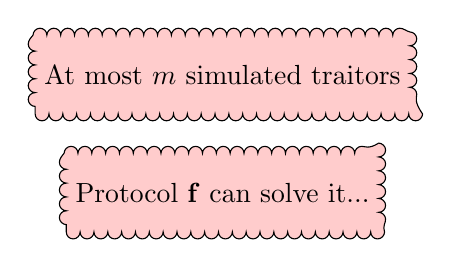
\begin{tikzpicture}[node distance=1.5cm]
  % First node
  \node [fill=red!20, draw, decorate, decoration={bumps, mirror}, 
         minimum height=1cm, align=center] (node1)
  {At most $m$ simulated traitors};

  % Second node placed below the first one
  \node [fill=red!20, draw, decorate, decoration={bumps, mirror}, 
         minimum height=1cm, align=center, below of=node1] (node2)
  {Protocol \textbf{f} can solve it...};
\end{tikzpicture}

\end{frame}
\begin{frame}{Impossibility Result \textcolor{red}{m>1}}
\begin{alertblock}{Assumption: \( m > 1 \) by contradiction}
\begin{itemize}
    \item If \( m > 1 \), then \( m = 1 \) 
    \item \( m = 1 \) can't be solved.
    \item(contradiction).
\end{itemize} 
\end{alertblock}

\end{frame}


\begin{frame}[plain]
\begin{tikzpicture}[remember picture, overlay]
    % Background Gradient
    \shade[bottom color=red!10, top color=white] 
        (current page.south west) rectangle (current page.north east);

    % Main Title with Shadow Effect
    \node[anchor=center, font=\Huge\bfseries\sffamily, 
          text=darkgray, 
          drop shadow={shadow xshift=0.5ex, shadow yshift=-0.5ex, opacity=0.5}] 
        at (current page.center) {\textbf{Oral Messages Fault\textcolor{red}{!!!}}};

    % Highlight Box with Rounded Corners
    \draw[ultra thick, red!70!black, rounded corners=8pt] 
        ($(current page.center) + (-5, 1.8)$) 
        rectangle 
        ($(current page.center) + (5, -1.8)$);
\end{tikzpicture}
\end{frame}


  
% 2105123 end




\begin{frame}{Solutions}
   \begin{columns}
       \begin{column}{.5\textwidth}
            \centering
           \huge \textcolor{Green}{So.. The Solution???}
       \end{column}
       \begin{column}{.5\textwidth}
            \vfill
            
            \includegraphics[width=0.5\linewidth]{image/solution.jpg}
       \end{column}
   \end{columns}
\end{frame}


\begin{frame}{Solutions 1:Oral Messages->OM(1)}
    \begin{tikzpicture}
     \node (king) at (2, 4) {\includegraphics[width=2cm]{image/king.png}};
    \node (soldier1) at (-2, 0) {\includegraphics[width=2cm]{image/Soldier.png}};
    \node (soldier2) at (2, 0) {\includegraphics[width=2cm]{image/Soldier.png}};
    \node (traitor) at (6, 0) {\includegraphics[width=1.5cm]{image/Traitor.png}};

    % Draw arrows and labels
    \draw[->, thick] (king) -- (soldier1) node[midway, above, text=blue] {ATTACK!};
    \draw[->, thick] (king) -- (soldier2) node[midway, above, text=blue] {ATTACK!};
    \draw[->, thick] (king) -- (traitor) node[midway, above , text=blue] {ATTACK!};
    \end{tikzpicture}
\end{frame}

\begin{frame}{OM(1)-3*OM(0)}
    \begin{tikzpicture}
     \node (king) at (3, 4) {\includegraphics[width=1cm]{image/king.png}};
    \node (soldier1) at (-2, 0) {\includegraphics[width=1.5cm]{image/Soldier.png}};
    \node (soldier2) at (3, 1) {\includegraphics[width=1.5cm]{image/Soldier.png}};
    \node (traitor) at (8, 0) {\includegraphics[width=1cm]{image/Traitor.png}};

    % Draw arrows and labels
    \draw[->, thick] (king) -- (soldier1) node[midway, above, text=blue] {ATTACK!};
    \draw[->, thick] (king) -- (soldier2) node[midway, above, text=blue] {ATTACK!};
    \draw[->, thick] (king) -- (traitor) node[midway, above , text=blue] {ATTACK!};

      \draw[->, thick, green, bend left=10] (soldier1) to node[midway, sloped, above] {\textbf{Attack!}} (soldier2);
      \draw[->, thick, green, bend left=10] (soldier2) to node[midway, sloped, below] {\textbf{Attack!}} (soldier1);
     \draw[->,thick, blue,bend right] (soldier1) to node[midway, sloped, above] {\textbf{Attack!}} (traitor);
     \draw[->,thick, red,bend left=20] (traitor) to node[midway, sloped, above] {\textbf{Retreat!}} (soldier1);
     \draw[->,thick, red,bend left=10] (traitor) to node[midway, sloped, above] {\textbf{Retreat!}} (soldier2);
        \draw[->,thick, green,bend left=10] (soldier2) to node[midway, sloped, above] {\textbf{Attack!}} (traitor);


    \end{tikzpicture}
\end{frame}
\setbeamercovered{transparent}
\begin{frame}{Oral Messages}
    \begin{itemize}
        \item \textcolor{Blue}{Intuition: }For every message \alert{M} received, we solve a smaller BGP containing all but the current commander to tell others  \alert{M} has been received.\pause
        \item \textbf{OM(m)} solvable for m traitors when 3m<n
    \end{itemize}
    \end{frame}
    
    \begin{frame}{Oral Messages}
     \only<1>{\textcolor{red}{Formally...}}
     \only<3>{\textcolor{Green}{Finally...}}
        \begin{itemize}
         \item \large OM(k)
            \begin{itemize}
                \item \textcolor{orange}{k==0}
                        \begin{itemize}
                            \item Commander sends value to everyone and everyone sends back the value they received
                            \pause
                        \end{itemize}
                \item \textcolor{orange}{k>0}
                        \begin{itemize}
                            \item Commander sends value to everyone
                            \item Everyone starts a smaller BGP \alert{OM(K-1)} where current Lieutenant becomes the new Commander
                            \item Everyone participated \textcolor{red}{n-1} \alert{OM(k-1)} and get \textcolor{red}{n-1} values, return the majority
                        \end{itemize}
            \end{itemize}
            \pause
    \end{itemize}
    \textbf{Complexity:}\textcolor{Blue}{ (n-1)*MC(OM(k-1)) + n-1 = O(n^m)}
\end{frame}

\begin{frame}{Solutions 2: Signed Messages}
    \begin{tikzpicture}
     \node (traitor) at (2, 4) {\includegraphics[width=1.5cm]{image/Traitor.png}};
    \node (soldier1) at (-2, 0) {\includegraphics[width=2cm]{image/Soldier.png}};
    \node (soldier2) at (6, 0) {\includegraphics[width=1.5cm]{image/Soldier.png}};

    % Draw arrows and labels
    \draw[->, thick,Green] (traitor) -- (soldier1) node[midway, above] {ATTACK!:0};
    \draw[->, thick,Red] (traitor) -- (soldier2) node[midway, above] {RETREAT!:0};
    \pause
     \draw[->,thick, Green] (soldier1) to node[midway, above] {\textbf{Attack!:0:1}} (soldier2);
        \draw[->,thick, Red,bend left=10] (soldier2) to node[midway, sloped, above] {\textbf{Retreat!:0:2}} (soldier1);
    \end{tikzpicture}
   \centerline{\only<2>{\textbf{V(1)==V(2)}}}
\centerline{\only<3>{\textbf{Choice(V(1))==Choice(V(2))}}}
\end{frame}

%2105129 start
\begin{frame}
    \frametitle{Minimum Number}
    \centering
    \includegraphics[width=\textwidth, height=\textheight, keepaspectratio]{image3/table.png}
\end{frame}


\begin{frame}
    \frametitle{Minimum Number}
    \centering
    \includegraphics[width=\textwidth, height=\textheight, keepaspectratio]{image3/table2.png}
\end{frame}

% Title


\begin{frame}{Partial Synchrony}
\begin{center}
    \textbf{\Huge Byzantine with digital signature in partial synchrony}
\end{center}

\vspace{1cm}  % Space between title and list

% Points
\begin{enumerate}
    \item synchronous 1/3 faults.

    \item Sound familiar?
    \item Assume there exist a protocol that can solve it.

\end{enumerate}

\end{frame}


% To fill the entire page with an image
\begin{frame}
    \frametitle{Partial Synchrony}
    \centering
    \includegraphics[width=\textwidth, height=\textheight, keepaspectratio]{image3/digital_signature.png}
\end{frame}



\begin{frame}{Practical Byzantine Fault Tolerance}
    \begin{itemize}
        \item Commander sends the value to every lieutenant
        \item Every lieutenant
        \begin{itemize}
            \item If it receives a new value \( v \), broadcast \texttt{(prepare, v)}
            \item If it receives \( 2f+1 \) \texttt{(prepare, v)}, broadcast \texttt{(commit, v)}
            \item If it receives \( 2f+1 \) \texttt{(commit, v)}, broadcast \texttt{(committed, v)}
            \item If it receives \( f+1 \) \texttt{(committed, v)}, broadcast \texttt{(committed, v)}
        \end{itemize}
        \item Ensure agreement
        \item Ensure liveness under a loyal commander \pause
        \item What if the commander is faulty?
        \begin{itemize}
            \item we need view change
        \end{itemize}

    \end{itemize}
\end{frame}




\begin{frame}{Minimum number required for which an $f$-resilient consensus protocol exists}
\centering
    \includegraphics[width=\textwidth, height=\textheight, keepaspectratio]{image3/table3.png}
    
\end{frame}


\begin{frame}{Application}

\centering
    \includegraphics[width=\textwidth, height=\textheight, keepaspectratio]{image3/application.jpg}


    
\end{frame}



\begin{frame}{Blockchain and Cryptocurrencies}
    \begin{columns}
        % Left Column (Text)
        \begin{column}{0.6\textwidth}
            \begin{itemize}
                \item \textbf{Problem Context:} In decentralized systems like Bitcoin, there are no central authorities to ensure all nodes agree on the state of the ledger.\pause
                \item \textbf{Solution:} Byzantine Fault Tolerance (BFT) algorithms ensure consensus despite malicious or faulty nodes.
            \end{itemize}
        \end{column}

        % Right Column (Images)
        \begin{column}{0.5\textwidth}
            \centering
            \includegraphics[width=1\textwidth]{image3/block-chain-digitalisation.jpg}\\[0.5cm]
            \includegraphics[width=1\textwidth]{image3/crypto.jpg}
        \end{column}
    \end{columns}
\end{frame}


\begin{frame}{Distributed Databases}
    \begin{columns}
        % Left Column (Text)
        \begin{column}{0.5\textwidth}
            \begin{itemize}
                \item Challenge is to ensure that all nodes have consistent data.\pause
                \item Byzantine fault tolerance can help maintain data consistency.
            \end{itemize}
        \end{column}

        % Right Column (Image)
        \begin{column}{0.5\textwidth}
            \centering
            \includegraphics[width=\textwidth]{image3/Distributed-database-system.png}
        \end{column}
    \end{columns}
\end{frame}




% Conclusion Slide
\begin{frame}{Conclusion}
    \begin{alertblock}{Key Takeaway}
        \textbf{Byzantine Fault Tolerance} (BFT) is the cornerstone of reliability in distributed systems. It enables:
        \begin{itemize}
            \item \textbf{Consensus:} Agreement among nodes, even with faulty or malicious participants.
            \item \textbf{Scalability:} Essential for decentralized systems like blockchain.
            \item \textbf{Resilience:} Smooth functioning in unpredictable environments.
        \end{itemize}
    \end{alertblock}
    \vfill
    \centering
    \textit{"By leveraging BFT protocols, we build systems that stand strong amidst failures."}
\end{frame}

% Thank You Slide
\begin{frame}{The End}

\centering
    \includegraphics[width=\textwidth, height=\textheight, keepaspectratio]{image3/Thankyou.jpg}



    
\end{frame}

\end{document}






